\documentclass[11pt,a4paper]{article}
\usepackage[utf8]{inputenc}
\usepackage{amsmath}
\usepackage{amsfonts}
\usepackage{amssymb}
\usepackage{graphicx}
\usepackage[english]{babel}
\usepackage[hidelinks]{hyperref}
\usepackage[backend=biber]{biblatex}
\bibliography{bib}

\author{Leo Touroul and Charles Bine}
\title{Structured compression}
\date{December 20, 2016}
\begin{document}

	\maketitle

	\section{Why structured compression?}
	Classifying datasets is an active field of research that allows to develop new technology mainly in image and sound recognition.
	
	
	The bottleneck when trying to classify datasets are the matrix multiplications happening in the neural networks used to classify the data.
	
	
	In order to tackle this bottleneck, and thus allow to run classifying models more rapidly, or at the same speed with cheaper/smaller components, one can use the concept of dimensionality reduction.
	
	
	Decreasing the dimensionality of the dataset being learned results in reducing the number of basic operations computed by the hardware and therefore speed up the classification.
	However, there is a limit to the number of dimension we can reduce the dataset we want to classify to. This paper will study more in depth the concept of dimensionality reduction using structured compressions.
	
	
	***explanation to have some content, matrix multiplication $O(n^3)$ time complexity ...***		
	
	\section{Setup experimental setup}
	To study the effect of dimensionality reduction using structured compression, we are going to use the classic MNIST dataset of handwritten digits. This dataset consists in grey-scale $28 \times 28$ images representing digits. Each image is associated with a label describing the digit represented by the image. Figure \ref{img:example_mnist_img} shows what an image from the dataset might look like. In that case, the associated label is "7".
	
	
	This dataset can be found at \url{http://yann.lecun.com/exdb/mnist/}. It is de facto split in 2 subsets : a training set (60k entries) and a test set (10k entries). We will devide the training set into 50k entries of training and 10k for validation. We decided to run our study on the dataset resulting of the merge of the training set and the dataset.
	
	
	***website Yann Lecun (+we need to do a bibliography? let's cite his HD3 triple spin paper)***.
	
	
	When we want to classify a dataset, we have to separate it in a training set and a test set. The training set is used to train the classifier (usually a neural network), and the test set is used to verify that the classification is working for general input, and is not overfitted to the training set. You can see this as making sure that the classifier didn't learn by heart the inputs contained in the training set.
	
	
	Here, we merged the training set and test set to then be able to choose the number of images used in the training set and the testing set. Originally, they respectively contained 50000 and 10000 images. Merging and spliting them as we wish allows us to have different proportion of input data in the training set and the dataset.
	
	
	***explanation MNIST, visualisation, there's an grey-scale imagine in the img/ folder***
	\begin{figure}
		\centering
		
\includegraphics[scale=0.7]{img/gYsJp.png}
		\caption{An example image from the MNIST dataset. In this case, the label is "7".}
		\label{img:example_mnist_img}
	\end{figure}
	
	The programming language used in this study is Python 3.5, allowing us to plug in powerful mathematical, statistical and plotting tools, on top of the new machine learning framework Tensorflow.
	
	
	This framework is a useful interface when we want to easily run the computations on GPU, which provides a huge speed up compared to running the computations on CPU because ***explanation to have some content***
	
	Structured compression:
	***explanation in depth***
	
	Non linear compression:
	***explanation, chaining, but we don't have any result on that, maybe we don't want to include this***
	
	\section{Results}
	Let's consider 2 datasets, one is the original one, let's call it \texttt{dataset\_original}, the second one is a transformed one.
	
	
	A transformation in our study is defined by a matrix multiplication to reduce the dimensionality, and a function applied element-wise. Therefore, a transformation is defined by 3 parameters, a kind of matrix used for the reduction, a target dimension, and a function.
	
	
	The notation \texttt{d\_m\_td\_f} represents the dataset where the matrix m with target dimension td and function f were applied.
	
	Let's consider a transformed dataset. The idea is that we are going to take a set of 2uples representing 2 images. For each 2uple, we are going to compute the distance (which one is to be determined) between those two points:
	
	\begin{enumerate}
		\item picked from the original, not transformed dataset,
		\item picked from the transformed data set
	\end{enumerate}

	Then we divide the second distance by the first distance. If the transformation keep the information contained in the dataset, it will allow us to classify the data using the transformed dataset (faster). We suppose this is true with the Euclidean distance, meaning that if the distances between two random points in the transformed dataset is roughly similar to the distance between the two original points in the original dataset, we won't have any problem classifying the data using the transformed dataset.
	
	
	Therefore, if we compute a huge number a quotient of distances, and we plot those results, we should expect a Gaussian with mean 1 and small variance for a transformation that keeps the properties of the original dataset and then allows us to classify it.
	
	
	***theory, JLT, inequality, epsilon***
	***practice: as we can see with the graphs, we can reduce the dimension up to (down to?) 16/32/64 ? without loosing much information regarding the euclidian distance***
	
	Here are the results for the various transformations:
	
	
	\subsection{Results}
	
	\begin{figure}
		\centering
		\begin{minipage}{.5\textwidth}
			\centering
			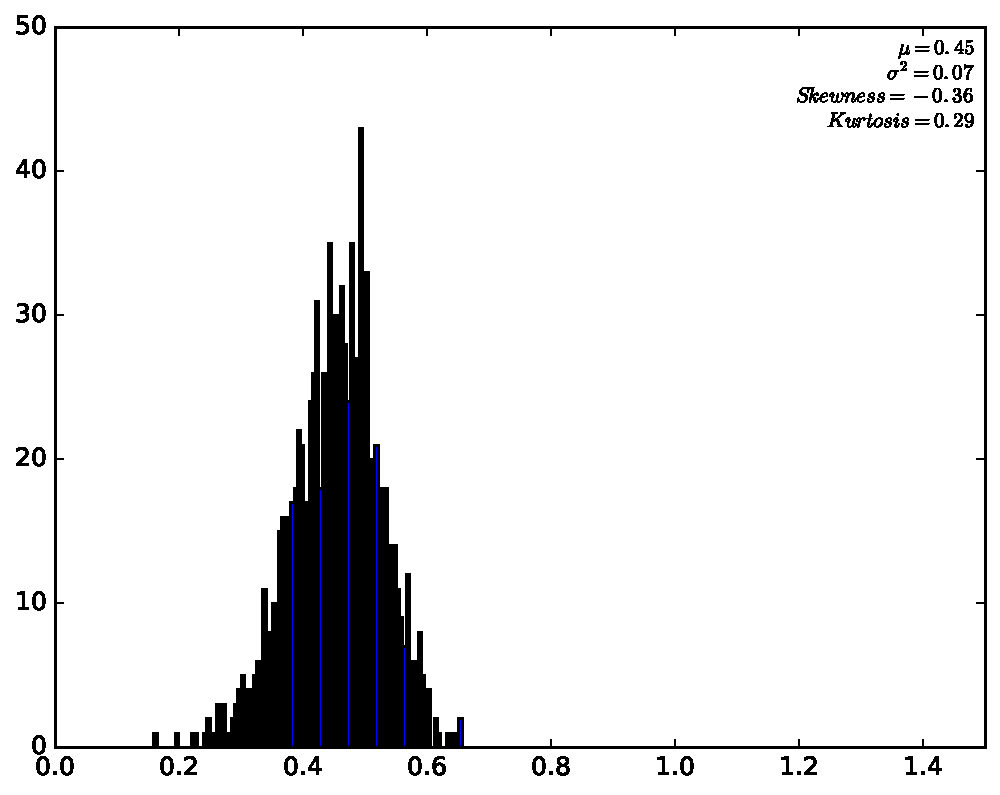
\includegraphics[width=.8\linewidth]{img/t_Drop_d_256_f_Identity.pdf}
			\caption{t\_Drop\_d\_256\_f\_Identity}
		\end{minipage}%
		\begin{minipage}{.5\textwidth}
			\centering
			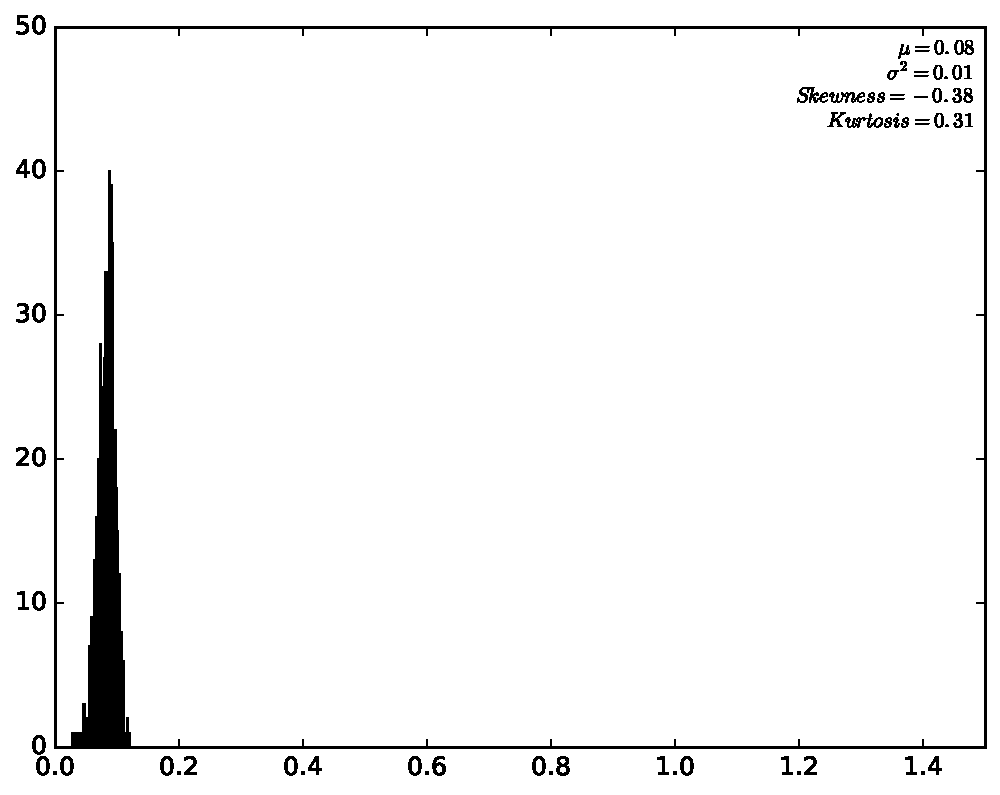
\includegraphics[width=0.8 \linewidth]{img/t_Drop_d_256_f_Sigmoid_diff.pdf}
			\caption{t\_Drop\_d\_256\_f\_Sigmoid diff}
			\label{fig:test2}
		\end{minipage}
	\end{figure}
	
	
	***all the images are in the folder img/, some grouped to be able to compre them, some indepedent, I let you choose which one you want to put. The quotient of distance when we apply a function is not 1, we can say that we would have to improve the nonlinear element-wise function and better tune them to get better results, or that maybe we should use the angular distance or another distance with those functions***
	
	\section{Classify}
	We used the framework tensorflow for the classification part. This framework provides useful neural networks out of the box with little need to be tuned and adapted. We first set up a simple softmax neural network to get familier with tensorflow's tensors and syntax. This feed forward neural network containing 1 hidden layer yields around 90\% of accuracy and runs in less than a second on CPU to classify MNIST pristine dataset.
	
	
	We then implemented a convolutional neural network with 2 feature maps layers, 2 pooling layers, and adding some drop out. This architecture yielded an satisfying 99.2\% of accuracy on MNIST pristine dataset but it took 30min of CPU time to train the model. On GPU, the computation time is expected to be a lot smaller but we unfortunately did not have access to a GPU compatible with cudNN (compute capability of 3.1 or 5.2)
	
	
	We therefore decided to run the classification using softmax feed forward neural networks. We were not able to run days of computation to get better accuracies using the second architecture. We still ran the second architecture on some transformed dataset to check if the speed up were working, and the accuracy wasn't lowered a lot. 
	
	
	Here are the results of the classification of the MNIST dataset, going through various pipelines, using a basic softmax feed forward neural network containing 1 hidden layer, with a learning rate of 0.5 and batch size of 100:
	
	Pipeline:
	\begin{itemize}
			\item Transform: Identity
			\item Target dimension: 784
			\item Function: Identity
			\item Result:
			\item Accuracy: 90.7\%
			\item Computation time: 1.xxxs
	\end{itemize}

	
	***repeat with all the various pipelines***
	
	
	\section{Problems Future improvements}
	The first obvious problem in this study is the lack of GPU access.
	
	
	An improvement, which we will implement as soon as we have access to a GPU with a CUDA compute capability of 5.2, would be to run the classifying part using the second architecture.
	This faster computation pipeline will allow us to run various training phases allowing us to first tune and find the optimal hyperparameters for this dataset.
	
	
	It will also allow us to extend the results to other datasets such as CIFAR-10 and CIFAR-100, which input images are a lot bigger than the one in MNIST, and where the complexity is significantly higher.
	
	
	Being able to run the classification part will allow us to plot the optimal accuracy as a function of the feature map sizes and the stride.
	
	
	Once the best parameters are found, we will run the classifying part on all the transformed datasets using various transformation, non linear functions, and even chaining the transformations.
	
	Another improvement would be to chain the various transformations and dimensionnality reductions pipelines and compare their efficiencies with those of one unique global dimensionnality reduction pipeline.
	
	
	\section{Conclusion}
	This study was a great way to understand in depth the classifying architecture yielding the best result so far in image and sound recognition (using convolutional neural networks), and the mechanisms associated with this architecture.
	
	
	It was also a great way to understand ho structured compression works, and how it allows to reduce the computation times, while still preserving the accuracy. This knowledge is important to either run the algorithms linked with artificial intelligence faster, or run them on less efficient pieces of hardware such as mobile phones.



	\nocite{*}
	\printbibliography


\end{document}



